\documentclass{book}
\usepackage{amsfonts}
\usepackage{amsmath}
\usepackage{graphicx}
\usepackage{epstopdf}
\usepackage{amssymb}
\usepackage{hyperref}
\usepackage{textcomp}
\usepackage{listings}
\usepackage{units}
\usepackage{color}

\definecolor{dkgreen}{rgb}{0,0.6,0}
\definecolor{gray}{rgb}{0.5,0.5,0.5}
\definecolor{mauve}{rgb}{0.58,0,0.82}

\lstset{frame=tb,
  language=Python,
  aboveskip=3mm,
  belowskip=3mm,
  showstringspaces=false,
  columns=flexible,
  basicstyle={\small\ttfamily},
  numbers=none,
  numberstyle=\tiny\color{gray},
  keywordstyle=\color{blue},
  commentstyle=\color{dkgreen},
  stringstyle=\color{mauve},
  breaklines=true,
  breakatwhitespace=true,
  tabsize=3, upquote=true}

\lstMakeShortInline[columns=fixed]|

\setcounter{chapter}{2}

\begin{document}

\chapter{Measurement and Uncertainty II}

I\ hope that by now you have been taught what a derivative is in your Math 112
class. But if not, we will learn what it is today. For our purposes, a
derivative is a slope of a line. You should recognize the equation of a
straight line as
\[
y=mx+b
\]
The slope $m$ can be written as
\[
m=\frac{dy}{dx}
\]
This is nothing magic. It is just a strange way to write $m.$ With the slope
written this way, the equation of the line could be written as
\[
y=\frac{dy}{dx}x+b
\]
But why $dy/dx$? Think of how we find a slope of a line. Back in junior high
school we called the slope the \textquotedblleft rise over
run.\textquotedblright\ That is, the change in $y$-value divided by the change
in the $x$-value.
\[
m=\frac{y_{2}-y_{2}}{x_{2}-x_{1}}
\]
In physics, we write the change in a variable using the greek letter delta,
$\Delta.$ So we could write the slope as
\[
m=\frac{y_{2}-y_{2}}{x_{2}-x_{1}}=\frac{\Delta y}{\Delta x}
\]
\ We need to get used to this delta notation, so let me write out $\Delta y$
\[
\Delta y=y_{2}-y_{1}
\]
and $\Delta x.$
\[
\Delta x=x_{2}-x_{1}
\]
So our straight line equation should be written
\[
y=\frac{\Delta y}{\Delta x}x+b
\]
but if we take $\Delta x$ to be very, very small it is customary to write the
$\Delta x$ as just $dx$ (I guess a \textquotedblleft d\textquotedblright\ is
smaller than a \textquotedblleft$\Delta$\textquotedblright). If this is not
familiar from Math 112, is should be by now from PH121 (if is not familiar at
all, call me over for help, but still don't panic--we are just writing slope
in a strange way).

In PH121 you have or will shortly learn that the velocity is the slope of the
plot of $x$ vs. $t,$ for example,
\[
y=\frac{1}{2}\frac{\text{m}}{\text{s}}t+1\text{m}
\]
is an equation giving the $y$ position of an object as a function of time.
Note that it is a straight line on a $y$ vs. $t$ plot.
\begin{center}
\fbox{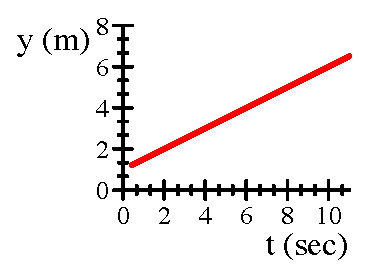
\includegraphics[
natheight=1.868000in,
natwidth=3.499900in,
height=1.868in,
width=3.4999in
]
{Lab3_figs/LineGraph.eps}
}
\end{center}
The slope of the line is
\[
\frac{dy}{dt}=\frac{1
\text{m}
}{2
\text{s}
}
\]
We can verify that this works by looking at the plot and noting that for every
two units of time, we go up one position unit. The slope is $1/2\frac{
\text{m}
}{
\text{s}
}.$

But not all curves are straight lines. What do we do with curves that, well, curve?

One idea is that we could split up the curve into little line segments, each
with its own slope. We can think of $dy/dt$ as an instantaneous slope, a slope
of one of the tiny line segments that make up our curve. This is the sort of
speed measurement that your speedometer gives. The speed might be different a
short time later. But right now the speed is, say, $0.5
\text{m}
/
\text{s}
.$

\begin{center}
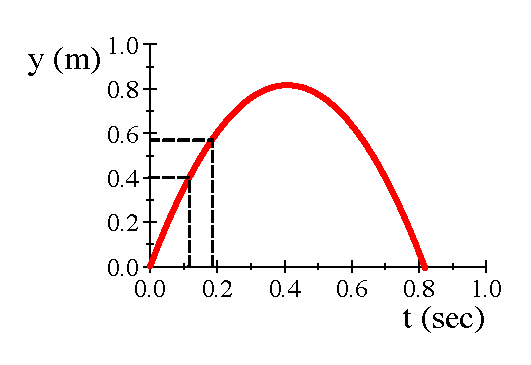
\includegraphics[
natheight=2.290000in,
natwidth=3.392700in,
height=2.3307in,
width=3.4385in
]
{Lab3_Figs/Parab_twopoints.eps}
\end{center}
Really, in defining an instantaneous slope we have assumed that the slope near
our point on the curve is essentially a straight line if $\Delta t$ is small enough.

We can use this idea to interpret our error calculations. Suppose I\ throw a
ball in the air with a initial speed of $4
\text{m}
/
\text{s}
$ straight up starting from $y_{o}=0$. From PH121 you have learned (or will
soon learn) that the equation for predicting how high the ball will go is
\[
y=y_{o}+v_{o}t+\frac{1}{2}at^{2}
\]
It says that starting at $y_{o}$ the ball will go higher depending on the
initial velocity, $v_{o},$ and the acceleration, $a.$ That make sense.

At a time, $t,$ the ball should be at
\[
y=0+4\frac{
\text{m}
}{
\text{s}
}t-\frac{1}{2}\left(  9.8\frac{
\text{m}
}{
\text{s}
^{2}}\right)  t^{2}
\]
where $a=-9.8\frac{
\text{m}
}{
\text{s}
^{2}}$ is the acceleration due to gravity. So, knowing this, I could predict
how high the ball would go if I\ pick a particular time, say, $0.15
\text{s}
.$ The result should be
\begin{align*}
y  & =0+4\frac{
\text{m}
}{
\text{s}
}\left(  0.15
\text{s}
\right)  -\frac{1}{2}\left(  9.8\frac{
\text{m}
}{
\text{s}
^{2}}\right)  \left(  0.15
\text{s}
\right)  ^{2}\\
& =0.489\,75
\text{m}
\end{align*}
This is shown in the next figure with a black line. Solving the equation for
$y$ is equivalent to drawing a line up to the curve, then from our spot on the
curve over to the $y$-axis to find the position.
\begin{center}
\fbox{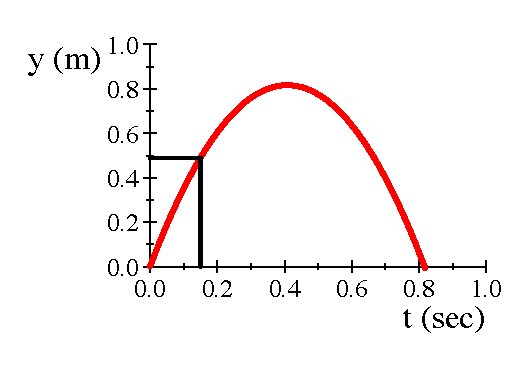
\includegraphics[
natheight=2.229500in,
natwidth=3.343400in,
height=2.2295in,
width=3.3434in
]
{Lab3_figs/Parab_onepoint.eps}
}
\end{center}


For our case we plot a line upward from $0.15
\text{s}
$ to the curve, and then plot a horizontal line from the intersection to the
$y$-axis. We can see that we get $4.9
\text{m}
.$ Suppose I try to verify this by taking a picture of the ball in flight at
$0.015
\text{s}
,$ but my stop watch is only good to $\pm0.005$ seconds. I try to take the
picture when the watch is at $0.015
\text{s}
,$ but I might have taken the picture at $0.01
\text{s}
$ or at $0.02
\text{s}
$ or anywhere in between. My time has some uncertainty. What does the
uncertainty in my stop watch time mean for the uncertainty in my $y$ value?

We can get a good approximation by graphically drawing vertical lines up from
$t_{\min}$ and $t_{\max}$ to the curve, and then extending horizontal lines
from the intersections to the $y$-axis. This gives us a $y_{\min}$ and
$y_{\max}.$ Our actual height could be anywhere in between these. This is a
way to view our uncertainty in $y.$
\begin{center}
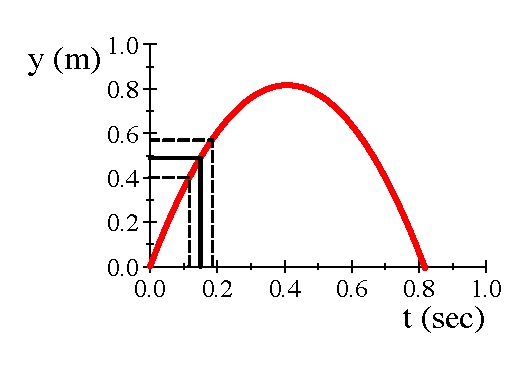
\includegraphics[
natheight=2.734500in,
natwidth=4.115600in,
height=2.7769in,
width=4.1658in
]
{Lab3_Figs/Parab_threepoints.eps}
\end{center}


We can use this idea to find a general way to calculate uncertainties. We
could define $\Delta t=t_{\max}-t_{\min}$. If our $\Delta t$ is small enough
(so we can write it just $dt$), the curve is essentially a straight line in
the region between $t_{\min}$ and $t_{\max}.$ So if we knew the slope of that
line (the derivative $dy/dt$) we could easily figure out the $y_{\max}$ and
$y_{\min}$ points to get our uncertainty range, at least if we stay near our
$t_{n}$ part of the curve. Recall that our uncertainty in $y $ using the
high/low method is
\[
\delta y=\frac{y_{\max}-y_{\min}}{2}=\frac{\Delta y}{2}
\]
Remembering that
\[
y=\frac{dy}{dt}t+b
\]
then
\begin{align*}
\Delta y  & =y_{\max}-y_{\min}\\
& =\frac{dy}{dt}t_{\max}+b-\frac{dy}{dt}t_{\min}-b\\
& =\frac{dy}{dt}\Delta t
\end{align*}
From your reading, you will recognize this as almost the uncertainty in a
function of one variable! But even if you don't recognize it, we can show that
this is true using our high/low method. The quantity $\Delta t$ is
\[
\Delta t=t_{\max}-t_{\min}
\]
so our uncertainty in $t$ would be
\[
\delta t=\frac{t_{\max}-t_{\min}}{2}=\frac{\Delta t}{2}
\]
then
\begin{align*}
\delta y  & =\frac{y_{\max}-y_{\min}}{2}\\
& =\frac{1}{2}\frac{dy}{dt}\Delta t\\
& =\frac{dy}{dt}\frac{\Delta t}{2}\\
& =\frac{dy}{dt}\delta t
\end{align*}
so
\[
\delta y=\frac{dy}{dt}\delta t
\]
So our uncertainty in $y$ is just the slope at our point on the curve
multiplied by our uncertainty in $t.$

But what if we have more than one variable? Say, we have a function $y(x,z),$
we essentially have a two dimensional slope. Think of a hill, you can go down
a hill in more than one direction. So we need slope parts for each direction
we can go.

But there is a fix we need to make to this equation that you won't learn for
several math classes to come. We want to have a slope in the $x$ and $z$
direction, but we want the slopes to be independent (if you have already taken
PH121, think of two dimensional motion problems, we split the problem into
components). The notation for this is
\[
\Delta y=\frac{\partial y}{\partial x}x+\frac{\partial y}{\partial z}z
\]
where
\[
\frac{\partial y}{\partial x}
\]
means the component of the slope just in the $x$ direction. We take a
derivative of the function $y,$ but assume only $x$ is a variable (treat $z$
and all $z$ terms with no $x^{\prime}s$ as constants). This lets us separate
the $x$ and $z$ parts. A special, one variable derivative like $\partial
y/\partial x$ is called a \emph{partial derivative} because you only take one
dimension of the derivative at a time. The reading from Chapter 3 uses this
type of derivative to find the general formula for error propagation. If we
wish to find the error in some general function $z\left(  x,y\right)  $ the
error is given by
\[
\delta y=\sqrt{\left(  \frac{\partial y}{\partial x}\right)  ^{2}\delta
x^{2}+\left(  \frac{\partial y}{\partial z}\right)  ^{2}\delta z^{2}}
\]
This looks a lot like our slope equation What we are doing is to assume the
function $y\left(  x,z\right)  $ is flat in a small region around the point we
are studying. then the function has a slope $\partial y/\partial x$ in the $x
$-direction, and $\partial y/\partial z$ in the $y$-direction. Each term like
\[
\left(  \frac{\partial y}{\partial x}\right)  \delta x
\]
gives how far off we could be in that direction (the $x$-direction in this
case). Remember that we have assumed that $y\left(  x,z\right)  $ is
essentially flat near our point of interest. The square root may be something
of a mystery, but remember what you have learned or are learning about adding
vectors in PH121. We add components of a vector to find the magnitude like
this
\[
V=\sqrt{V_{x}^{2}+V_{y}^{2}}
\]
This comes from the Pythagorean theorem. The $x$ and $y$ parts of the vector
form two sides of a triangle. We want the remaining side. So we use the
Pythagorean theorem to find the length of the remaining side.

We are doing the same for our small uncertainty lengths. We are just adding
the $x$ and the $y$ components of the error. We could write our error formula
for the general case of a function $f$, that depends on $N$ different
variables.
\[
\delta f=\sqrt{\sum_{i=1}^{N}\left(  \frac{\partial f}{\partial x_{i}}\right)
^{2}\delta x_{i}^{2}}
\]
We will use this formula a lot, so make sure you understand what it means (ask
your instructor for help if it is not clear).

\section{How do we find the slope?}

But now we have an equation in terms of slope written as $dy/dx$ or $dy/dz$,
but how would we ever find these slops? Your calculus class has or will teach
you this. So we will just give you some quick formulas that will work for most
equations, then you can ask your instructor if you have something odd like an
$\arctan$ function.

For polynomials like,
\[
f\left(  x\right)  =ax^{2}+bx+c
\]
each term follows the rule
\[
\frac{d}{dx}\left(  ax^{n}\right)  =anx^{n-1}
\]
that is, if I have a constant, $a,$ times $x^{n}$ the slope of this curve is
the constant, $a,$ times the power, $n,$ times $x$ to the $n-1$ power.

Let's take an example. What is the slope of the function $y=5x^{3}?$

\[
\frac{d}{dx}\left(  5x^{3}\right)  =\left(  5\right)  \left(  3\right)
x^{3-1}=15x^{2}
\]


How about finding the slope of $y=7x^{2}-2x+1$

\[
\frac{d}{dx}\left(  7x^{2}-2x+1\right)  =\left(  7\right)  \left(  2\right)
x^{1}-\left(  2\right)  (1)x^{0}+0
\]
The last term illustrates that the slope of a constant is zero. That makes
sense. Constants don't change. So the change in $y$ just due to the last term
$(1)$ should be zero. We also remember $x^{0}=1.$ So we are left with
\[
\frac{d}{dx}\left(  7x^{2}-2x+1\right)  =14x-2
\]


This one rule will take care of most of our functions for now. Let's try one
more, say $y=x^{\frac{1}{2}}$
\[
\frac{d}{dx}\left(  x^{\frac{1}{2}}\right)  =\frac{1}{2}x^{-\frac{1}{2}}
\]
This could be written as
\[
\frac{d}{dx}\left(  \sqrt{x}\right)  =\frac{1}{2}\frac{1}{\sqrt{x}}
\]
So we see we can handle square roots with this rule.

\section{Tie to statistics}

We need to tie our statistical ideas into what we have learned about error
propagation. Lets go back to our function $f\left(  x,y\right)  $ the error is
given by
\[
\delta f=\sqrt{\left(  \frac{\partial f}{\partial x}\right)  ^{2}\delta
x^{2}+\left(  \frac{\partial f}{\partial z}\right)  ^{2}\delta z^{2}}
\]
but now we know we could express this in terms of standard deviations
(provided you don't need to ensure all data are within your uncertainty
range). We can write our uncertainties as
\[
\sigma_{f}=\sqrt{\left(  \frac{\partial f}{\partial x}\right)  ^{2}\sigma
_{x}^{2}+\left(  \frac{\partial f}{\partial z}\right)  ^{2}\sigma_{z}^{2}}
\]


We can use this to show that the standard deviation of the mean (the best
estimate of our uncertainty) is given by

\[
\sigma_{\bar{x}}=\frac{\sigma_{x}}{\sqrt{N}}
\]
Think of calculating a mean value
\[
\bar{x}=\frac{x_{1}+x_{2}+\cdots x_{N}}{N}
\]
We can find the uncertainty in this function $\sigma_{\bar{x}}$
\[
\sigma_{\bar{x}}=\sqrt{\left(  \frac{\partial\bar{x}}{\partial x_{1}}\right)
^{2}\sigma_{x_{1}}^{2}+\left(  \frac{\partial\bar{x}}{\partial x_{2}}\right)
^{2}\sigma_{x_{2}}^{2}+\cdots+\left(  \frac{\partial\bar{x}}{\partial x_{N}
}\right)  ^{2}\sigma_{x_{N}}^{2}}
\]
You see we just take the partial derivative of our function $\bar{x}$ with
respect to each of the variables $x_{i}$ and multiply by the uncertainty in
that variable written now as a standard deviation $\sigma_{i}.$

For this special case, all of the $x_{i}$ are the same (we are measuring the
same value over and over in taking an average) and all of the $\sigma_{i}$ are
the same so we just have
\[
\sigma_{\bar{x}}=\sqrt{N\left(  \frac{\partial\bar{x}}{\partial x_{1}}\right)
^{2}\sigma_{x_{1}}^{2}}
\]
and we can take the derivative using our rule. Only $x_{1}$ is a variable, so
we can write the average $\bar{x}$ as
\[
\bar{x}=\frac{x_{1}}{N}+\frac{x_{2}+\cdots x_{N}}{N}
\]
This is a polynomial! The first term is $\frac{1}{N}x_{1}$ and the whole
second term is a constant if we take a partial derivitive with respect to
$x_{1}$. The derivative is
\begin{align*}
\frac{\partial\bar{x}}{\partial x_{1}}  & =\frac{\partial}{\partial x_{1}
}\left(  \frac{x_{1}+x_{2}+\cdots x_{N}}{N}\right) \\
& =\frac{1}{N}x_{1}^{0}+0\\
& =\frac{1}{N}
\end{align*}
so our statistical error function is just
\begin{align*}
\sigma_{\bar{x}}  & =\sqrt{N\left(  \frac{1}{N}\right)  ^{2}\sigma_{x_{1}}
^{2}}\\
& =\sqrt{\frac{\sigma_{x_{1}}^{2}}{N}}\\
& =\frac{\sigma_{x_{1}}}{\sqrt{N}}
\end{align*}
or, since all the $\sigma_{x_{i}}$ are the same, we can just write this as
\[
\sigma_{\bar{x}}=\frac{\sigma_{x}}{\sqrt{N}}
\]


Notice that in this example we had many $x_{i}$ and that to find the
uncertainty we just extended our equation from two variables
\[
\sigma_{f}=\sqrt{\left(  \frac{\partial f}{\partial x}\right)  ^{2}\sigma
_{x}^{2}+\left(  \frac{\partial f}{\partial z}\right)  ^{2}\sigma_{z}^{2}}
\]
to $N$ variables
\[
\sigma_{f}=\sqrt{\sum_{i=1}^{N}\left(  \frac{\partial f}{\partial x_{i}
}\right)  ^{2}\sigma_{i}^{2}}
\]


In this special case, we were trying to show a special result, but we can do
this for any function with any number of variables. If your function is
complicated, you just need to take more partial derivative terms under the
square root.

\pagebreak

\section{Assignment}

Measure the acceleration due to gravity, $g,$ four different ways. For each
case, determine an experimental value for $g$ along with its uncertainty.
Record how you find $g$ and its uncertainty for each method in your lab
notebook. Try to obtain the best value you can for each method.

\subsection{Method 1: Timing a ball drop}

Using a stop watch and a tennis ball, drop the ball over a known height and
determine a value for $g.$

\subsection{Method 2: Using a pendulum}

You will learn in PH123 that a pendulum oscillates back and forth at a certain
rate. If you don't plan to take PH123, you still know that the pendulum of a
grandfather clock sets the rate at which the clock will run. The time it takes
the pendulum to go back and forth is called the \emph{period of oscillation}.
That period is given by the following equation
\[
T=2\pi\sqrt{\frac{L}{g}}
\]
where for some reason the letter $T$ stands for period, and $L$ is the length
of the pendulum string, and $g$ is the acceleration due to gravity. Build your
pendulum, and measure the period of oscillation using a photogate. From this
obtain a value for $g.$

\subsection{Plot Your Results}

A spreadsheet program (e.g. MS Excel or LibreCalc) can graph data, and so can
a piece of software on our lab computers named LoggerPro. You may know how to
make a graph in one of these tools.

In this class, we are using python, so you should try making your plot in python.  Last week, we used matplotlib to build a histogram. The command for building a plot with errorbars is very similar.  Assuming that you've imported matplotlib as |plt|, the command looks like this:
\begin{lstlisting}[language=python]
plt.errorbar(x,y,xerr=xerr_variable,yerr=yerr_variable,fmt='o')
\end{lstlisting}
|xerr| and |yerr| are optional commands. If you you want error bars in the x direction, and you've saved the size of your x error in the variable |my_x_err|, sometime after your x and y lists, you'd include the command |xerr=my_x_err|. If you don't have any x-error bars, leave out |xerr|.

  Try to make a plot of the two different values you found for $g$, with errorbars, by using the |errorbar| command and by borrowing and adapting parts of last week's program. The commands for labeling the axes, title, etc. for an |errorbar| plot are the same as the commands for a histogram.

\subsection{Method 3: High Speed Camera}

Take high speed video of a falling ball. Important things to do as you take your video:
\begin{itemize}
\item Include a meter stick or something of known length in your video. 
\item Try not to move the camera as you take the video
\item If you record with high speed on a cell phone, make sure that the frame rate is constant.  Many smart phones will let you start in real time, slow it down, then speed it up again.  Do not do this.
\end{itemize}




Use either the \emph{Logger Pro} or \emph{Tracker} software to analyze the
video. Tracker has an autotracking option that can be very helpful if your ball does not blend into the background of your video. The steps to do this in Logger Pro are outlined in the Logger Pro help under
``video analysis."  The steps to do this in Tracker are on their web page under video tutorials.  ``Tracker Quick Start" gives a short version (2.5 min.). ``Getting Started with Tracker" has a longer version.

Fit a curve to your data that comes from the video. From you PH121 experience
you know that the acceleration due to gravity is constant, so we can use the
equation
\[
y=y_{o}+v_{o}t+\frac{1}{2}at^{2}
\]
to indicate the type of curve to use for our fit. If you have trouble finding
the curve fit function in Logger Pro or Tracker, or have trouble using Logger Pro or Tracker, call
your instructor over.




\end{document}
